\section{Architecture}
\label{sec:architecture}
The architecture for this project was designed to be easily expandable for future work. The raw design is shown in figure \ref{fig:architecture}. 
\begin{figure}[!ht]
	\caption{A UML depicting the raw architecture implemented for this project. }
	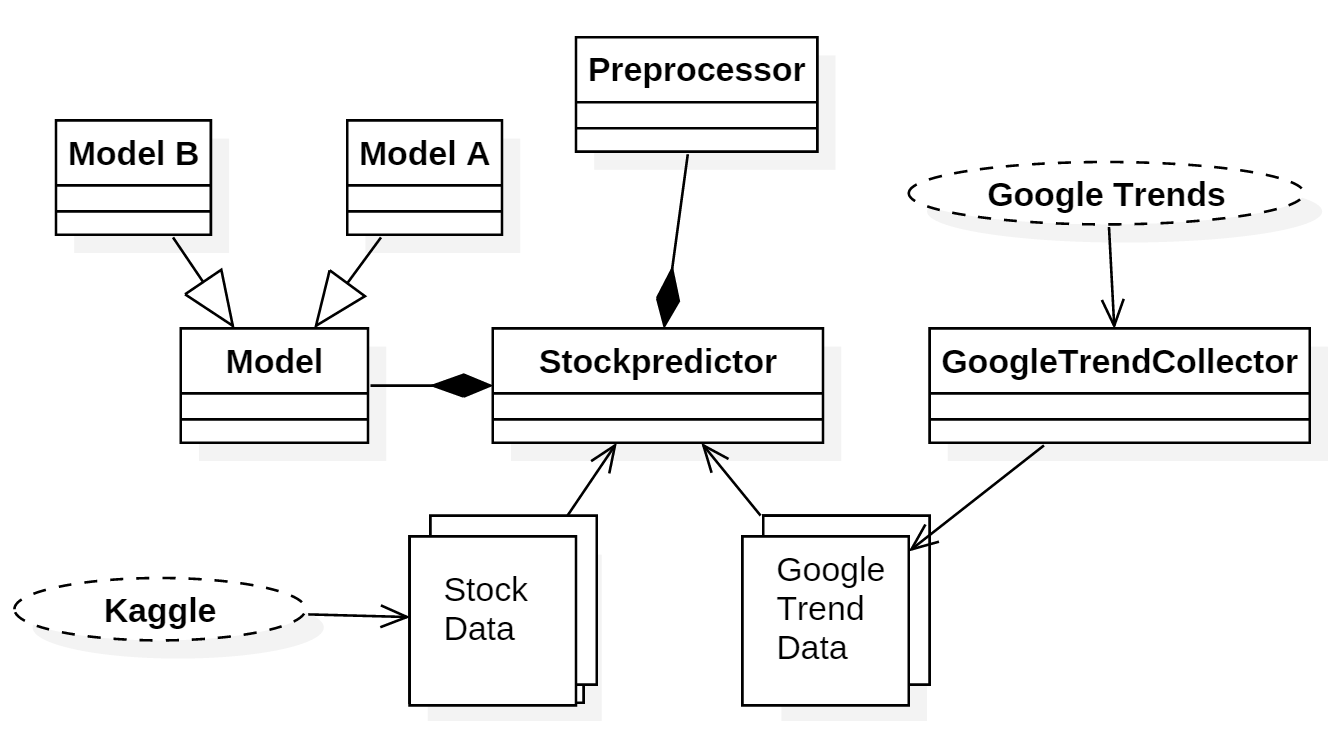
\includegraphics[width=0.95\linewidth]{images/architecture.png}
	\label{fig:architecture}
\end{figure}
\\
The \textit{GoogleTrendCollector} gathers all data regarding the information provided by the Google trends service as described in section \ref{subsec:gtdata}. The stock data, however, is just downloaded from \textit{kaggle}. 
\\
Within the \textit{Preprocessor} class functions to read raw stock and Google trends data from csv-files as well as the zero centering are implemented. Additionally, it transforms the raw data into a more useful shape. The functionality to save, read and delete the preprocessed data is also provided by the \textit{Preprocessor} class. 
\\
By extracting the learning model into a separate class the architecture becomes flexible regarding the use of different models. This also greatly reduces duplicity of code within the entire project. As there are basic functions used by all kind of learning models, an abstract class \textit{Model} was defined. It provides basic functionality and enforces inheriting classes to implement other necessary methods. For example, the functions of saving and restoring a trained model is used by every kind of learning model, wherefore it is implemented in the abstract parent class. On the other hand, functions like training and predicting may vary between different types of models. Hence, such functions are only defined in the \textit{Model} class and need to be implemented in any inheriting model class. The used model for this project is explained in more detail in section \ref{sec:model}. 
\\
The \textit{Stockpredictor} class serves as the central part of the whole structure. It uses an object of the \textit{StockpredictorConfig} to configure settings like the learning rate and the number of epochs for the training as well as the used count of folds \textit{k} for the cross validation. An object of the \textit{Model} is also passed as a parameter to the \textit{Stockpredictor} constructor. During the training process this model is being used. Also, an already trained model can be passed to the \textit{Stockpredictor} for further training or prediction. The train function of the \textit{Stockpredictor} partitions all available data. Also, the epoch loop as well as the loop of the k fold cross validation is implemented at this position. The train method of the respective model, however, executes the actual training. This also applies to the predict function. Although the \textit{Stockpredictor} manages all available data, it delegates the preprocessing of raw data to the \textit{Preprocessor} class. 
\\
For this project \textit{TensorFlow}, an open-source library for machine learnig, is used. The previously described classes are implemented using the programming language \textit{Python}. The access to \textit{TensorFlow} is therefore facilitated by using its \textit{Python}-API. Packages like \textit{numpy} and \textit{jsonmerge} are used additionally to simplify certain operations. 